\documentclass[twoside]{article}
\usepackage{float} 
\usepackage{bookmark}
\usepackage{titlesec}
\usepackage{titling}
\usepackage{graphicx}
\usepackage{tikz}
\usepackage{pgfplots}
\usepackage{caption}
\usepackage{multirow}
\usepackage{fancyhdr} 
\usepackage{graphicx}
\usepackage{hyperref}
\usepackage{titlesec}
\usepackage{natbib}
\usepackage{amsmath}
\usepackage{amsthm}
\usepackage{amssymb}
\usepackage{parskip}
\usepackage[utf8]{inputenc}
\usepackage{multicol}
\usepackage{csvsimple}
\usepackage{longtable}
\usepackage{textgreek}
\usepackage{listings}
\usepackage{booktabs}



\title{\textbf{A Laboratory Study on Recombinant GFP Expression and Characterization}}
\author{Rahul Chavan}
\markboth{Recombinant Expression and Purification of GFP}{\thepage}
\date{\today}

\pagestyle{fancy}
\fancyhf{}
\fancyhead[LO,RE]{\leftmark}
\fancyfoot[C]{\thepage}


\usepackage[left=1in, right=1in, top=1in, bottom=1in]{geometry}
\renewcommand{\maketitle}{
 \begin{center}
    
        \includegraphics[width=2cm]{IISc_Master_Seal_Black.jpg}
        \vspace{0.5cm}

        \Large
        \textbf{\thetitle}
        
        \vspace{0.5cm}
        
        \Large
        \theauthor

        \small{Bachelor of Science (Research), Indian Institute of Science, \href{mailto:rahulchavan@iisc.ac.in}{rahulchavan@iisc.ac.in}}
        
        \vspace{0.2cm}
        
        \large
        \thedate

        \vspace{0.5cm}

        \markboth{Recombinant Expression and Purification of GFP}{\thepage}

        \hrule  
        
    \end{center}
}

\pgfplotsset{compat=1.18}
\begin{document}
\maketitle

%We have done a continuous lab project on recombinant expression, purification and primary characterization of protein in this course. 
%Please prepare a succinct report with any journal format (General format should have, Title, Abstract, Introduction, Materials and methods, results and discussion, followed by references). 
%Please make sure that the submitted report has your respective TA name, so that they can find your reports easily. 

%cysteine disulfide bonds hence reducing agent is used to break the disulfide bonds.
%The purified protein was charecterized by measuring its absorbance and flourescence spectra, confirming its identity via SDS-PAGE, and Western Blotting.

% we expressed the protein
% we purified by ni nta affinity chromatography
% we checked on sds to see if the protein is present
% we dialysed it
% branford assay to check the concentration
% we checked the effect of temperature
% we did western blot to confirm our results
% pPROEx-Htb (has 6x-Histag, IPTG inducible trc promoter, and ampicillin resistance gene)


\begin{abstract}
Green Fluorescent Protein (GFP) is an invaluable tool in molecular and cell biology due to its unique fluorescent properties.
This continuous lab project aimed to express, purify, and charecterize GFP using recombinant DNA technology. The GFP gene was cloned into 
an expression vector and transformed \textit{E. coli} cells for protein production. Following induction 
with Isopropyl $\beta$-D-1-thiogalactopyranoside (IPTG), the cells were lysed and the GFP was purified using Ni-NTA affinity chromatography.
The purified protein was charecterized by confirming its identity via SDS-PAGE, and Western Blotting.
Additionally, the purified GFP was used to determine its concentration using the Bradford assay after dialysis.
The results demonstrated successful expression and purification of GFP, as well as its charecterization.
This project provides a foundational understanding of recombinant protein expression and purification techniques and lays the groundwork
for further studies on GFP and other proteins.
\end{abstract}


\begin{multicols}{2}

\subsection*{Introduction}
Green Fluorescent Protein (GFP), originally isolated from the jellyfish \textit{Aequorea victoria}, has revolutionized the field of 
molecular and cell biology since its discovery in the 1960s. This protein has been used for protein tagging,
in examining gene expression, and in various biological selections. GFP's popularity stems from its ability to be 
genetically fused to other proteins of interest without compromising their function, allowing us to 
visualize their localization and dynamics within living cells.

In this project, we aimed to express, purify, and characterize GFP using recombinant techniques. 
The recombinant expression of GFP involved cloning the GFP gene into an expression vector (pPROEx-Htb), followed by 
transformation into into BL21 Arctic Express$^{TM}$ strain of \textit{E. coli} cells for protein production. After induction with Isopropyl 
$\beta$-D-1-thiogalactopyranoside (IPTG), cells were lysed, and GFP was purified using Ni-NTA affinity chromatography. 
The isolated protein was also charecterized by confirming its identity via SDS-PAGE
The isolated protein was then subjected to dialysis to obatin a purified protein product which was then analysed using 
Bradford assay to measure the concentration of the protein.
The purified GFP was also charecterized by western blotting to confirm the results obtained from SDS-PAGE.

This project provides a hands-on approach to understanding the principles of recombinant protein expression, 
purification, and characterization, with GFP serving as a model protein. By successfully expressing and 
purifying GFP, we demonstrate the applicability of recombinant techniques in producing functional 
proteins for diverse research purposes.


\subsection*{Materials and Methods}

\textbf{Expression of Recombinant GFP:}


After the GFP gene was cloned into the pPROEx-Htb expression vector, the construct was transformed into 
BL21 Arctic Express$^{TM}$ cells. A single colony harboring the GFP expression construct was inoculated 
into 5 mL of LB broth containing 5 $\mu$L antibiotic Add 5 $\mu$L of antibiotic to 5 ml of LB broth
(Ampicilin(100$\mu$g/ml) and gentamycin (50$\mu$g/ml) is used for producing GFP), and grown overnight at 37°C with shaking. 
The overnight culture was diluted 1:100 into fresh LB broth supplemented with 200 $\mu$L of antibiotic (Ampicilin (100$\mu$g/ml), Gentamycin (50$\mu$g/ml)) 
for 200mL and grown at 37°C with shaking 
until reaching an optical density at 600 nm (OD600) of approximately 0.6-0.8. 
Expression of GFP was induced by adding Isopropyl $\beta$-D-1-thiogalactopyranoside (IPTG) 
to a final working concentration of 0.5-1mM, and the culture was incubated overnight at 11°C with shaking.

\begin{figure}[H]
    \centering
    \includegraphics[angle=270,width=0.25\textwidth]{Secondary_culture.jpg}
    \caption{Secondary culture for GFP expression}
    \label{fig:Secondary_culture}
\end{figure}

\textbf{Cell Lysis and Protein Extraction:}

Cells were harvested by pellet the cells at 3500 rpm for 10 minutes at 4°C. 
The cell pellet was resuspended in lysis buffer made of 50 mM Tris pH 8.0, 300 mM NaCl, 
Benzamidine 1mM, PMSF 1mM supplemented with lysozyme and protease inhibitors. 
Cell lysis was achieved by sonication on ice at 50\% amplitude for 5 minutes with 1s on and 2s off.
The sonication was repeated 5 times and the cell lysate was centrifuged at 12,000 rpm for 30 minutes at 4°C to separate the soluble fraction containing GFP from insoluble cell debris.




\textbf{Purification of GFP:}

The cleared lysate was loaded onto a Ni-NTA affinity chromatography column pre-equilibrated with lysis buffer, and incubated overnight at 4°C with gentle shaking. 
The column was unloaded (flowthrough collected) washed with wash buffer A (20m MTris pH 8.0, 300 mM NaCl, 20 mM Imidazole) to remove nonspecifically bound proteins, 
and then with wash buffer B (20 mM Tris pH 8.0, 300 mM NaCl, 40 mM Imidazole) and GFP was eluted using elution buffer (50 mM Tris pH 8.0, 300 mM NaCl and 250 mM Imidazole).
The washing was done 3 times each and elution was carried out until the colour of GFP disappeared from the column.

\begin{figure}[H]
    \centering
    \includegraphics[angle=270,width=0.3\textwidth]{Ni-NTA purification.jpg}
    \caption{Ni-NTA column}
    \label{fig:Ni-NTA_column}
\end{figure}



\textbf{Protein Purification Analysis:}

\textbf{SDS-PAGE} was performed to visualize the purified GFP. 
20 $\mu$L of the purified GFP samples were prepared with 1X SDS loading dye, boiled for 5 minutes at 95°C, and loaded onto a SDS-PAGE gel.
The gel was stained with CBB stain (CBB R-250 .25\%, Distilled water 50\%, Methanol 40\%, Glacial acetic acid 10\%) to visualize the protein bands.
The gel was then de-stained with destaining solution (Distilled water 50\%, Methanol 40\%, Glacial acetic acid 10\%).

\begin{figure}[H]
    \centering
    \includegraphics[angle=270,width=0.3\textwidth]{Gelrun.jpg}
    \caption{SDS-PAGE}
    \label{fig:SDS-PAGE}  
\end{figure}


The protein samples were then dialysed against 1L of dialysis buffer (50 mM Tris pH 8.0, 50 mM NaCl, 50\% glycerol) for overnight 
hours at 4°C with shaking to remove imidazole and other contaminants.

\begin{figure}[H]
    \centering
    \includegraphics[width=0.4\textwidth]{Dialysis.jpg}
    \caption{Dialysis of purified GFP}
    \label{fig:Dialysis}
\end{figure}

The concentration of the purified GFP was determined using the \textbf{Bradford assay}.
The Bradford reagent was prepared by preparing 5.0 ml of 1X Bradford Reagent by adding 1.0 ml of 5X stock solution (50 mg of 
Coomassie Brilliant Blue G-250, 47 ml of 100\% Methanol and 50 ml of 85\% Phosphoric Acid to the final volume of 100 ml) and 4.0 ml of distilled water.
A standard curve was prepared using Bovine Serum Albumin (BSA) as the standard protein, 
and the absorbance of the GFP samples was measured at 595 nm using a spectrophotometer by adding 5 $\mu$L
of the protein sample to 1X Bradford reagent.

\begin{figure}[H]
    \centering
    \includegraphics[width=0.4\textwidth]{Bradford.jpg}
    \caption{Bradford assay for GFP concentration}
    \label{fig:Bradford_assay}
\end{figure}

\textbf{Western Blotting} was performed to confirm the results obtained from SDS-PAGE.
The purified GFP was separated on a 12\% SDS-PAGE gel and transferred to a PVDF membrane using a semi-dry transfer apparatus.
The transfer buffer contained 25 mM Tris pH 8.3, 192 mM Glycine, and 20\% methanol.
The membrane was then blocked with 5\% BSA in TBST (Tris-buffered saline with 0.1\% Tween 20) for 1 hour at room temperature on rocker,
and then incubated with anti-His antibody (1:2000 dilution) overnight at 4°C after washing with TBST.
The membrane was washed with TBST and incubated with HRP-conjugated secondary antibody (1:5000 dilution) for 1 hour at room temperature.
The membrane was washed with TBST and developed using DAB solution. This was done by adding 1ml of 20X stock DAB solution and 2 $\mu$L of 30\% H$_2$O$_2$ to 20 ml of 25mM Tris pH 7.5, 
150mM NaCl. The membrane was then incubated in the DAB solution until brown precipitate bands appeared.

\begin{figure}[H]
    \centering
    \includegraphics[width=0.4\textwidth]{Western_membrane.jpg}
    \caption{Western blotting of purified GFP}
    \label{fig:Western_blotting}
\end{figure}

\textbf{Effect of Temperature on GFP Stability:}
The effect of temperature on protein folding and stability was determined by incubating the purified GFP at different temperatures 
(11°C and 37°C) and samples were collected after every 30 minutes for 2 hours. The samples were then subjected to the spectrophotometer
to measure the fluorescence intensity. The OD of the samples were also measured.


\subsection*{Results}

\textbf{Fexpression of Recombinant GFP:}

The GFP gene was successfully cloned into the pPROEx-Htb expression vector and transformed into BL21 Arctic Express$^{TM}$ cells for protein production.
The expression of GFP was induced by IPTG, and the cells when pelletted after overnight incubation
showed a green colour indicating the expression of GFP. This shows that the chaperoins present in the BL21 Arctic Express$^{TM}$ cells helped in the proper folding of the GFP protein.


\begin{figure}[H]
    \centering
    \includegraphics[angle=270,width=0.2\textwidth]{Cell pellet.jpg}
    \caption{Cell pellet}
    \label{fig:Cell_Lysis}
\end{figure}

\textbf{SDS-PAGE:}
The GFP was purified using Ni-NTA affinity chromatography, and the purified protein was visualized using SDS-PAGE.
The SDS-PAGE gel showed a single band at the expected molecular weight of GFP (27 kDa), indicating successful purification of the protein.


\begin{figure}[H]
    \centering
    \includegraphics[width=0.4\textwidth]{SDSPAGEgel.jpg}
    \caption{SDS-PAGE of purified GFP}
    \label{fig:SDS-PAGE GEL}
\end{figure}

\textbf{Bradford Assay:}
The concentration of the purified GFP was determined using the Bradford assay. 
The standard curve was prepared using BSA as the standard protein,
and the absorbance of the GFP samples was measured at 595 nm using a spectrophotometer.

\begin{figure}[H]
    \centering
    \includegraphics[width=0.4\textwidth]{Bradford table.jpg}
    \caption{Bradford assay data}
    \label{fig:Bradford_assay_data}
\end{figure}



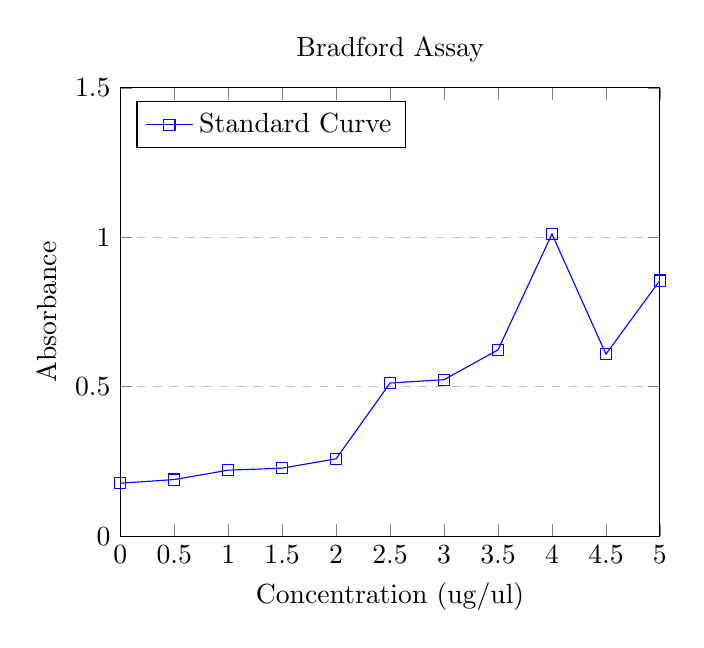
\begin{tikzpicture}
    \begin{axis}[
        title={Bradford Assay},
        xlabel={Concentration (ug/ul)},
        ylabel={Absorbance},
        xmin=0, xmax=5,
        ymin=0, ymax=1.5,
        xtick={0,0.5,1,1.5,2,2.5,3,3.5,4,4.5,5},
        ytick={0,0.5,1,1.5},
        legend pos=north west,
        ymajorgrids=true,
        grid style=dashed,
    ]
    
    \addplot[
        color=blue,
        mark=square,
        ]
        coordinates {
        (0,0.177267)(0.5,0.1895)(1,0.220867)(1.5,0.2276)(2,0.258967)(2.5,0.5125)(3,0.523667)(3.5,0.6233)(4,1.011323)(4.5,0.609167)(5,0.8554)
        };
        \legend{Standard Curve}
        ;
    \end{axis}
\end{tikzpicture}

\begin{figure}[H]
    \centering
    \includegraphics[width=0.4\textwidth]{Bradford plot.jpg}
    \caption{Bradford assay curve fit}
    \label{fig:Bradford_assay_plot}
\end{figure}

From the plot we can extrapolate that the concentration of the sample is 1.237 $\mu$g/ul.
Hence, the concentration of the purified GFP is 1.237 $\mu$g/ul.    

\textbf{Effect of Temperature:}
The study provided insights into the effect of temperature on the stability of GFP.
The fluorescence intensity and OD of the purified GFP was measured at different temperatures (11°C and 37°C) over a period of 2 hours.
The results showed that the fluorescence per cell intensity (which was calculated by dividing the fluorescence intensity by the OD)
of GFP decreased with increasing temperature, indicating that GFP is more stable at lower temperatures.

\textbf{OD measurements:}

\begin{tabular}{|c|c|c|}
    \hline
    Time (min) & 37 degrees & 11 degrees \\
    \hline
    0 & 0.1916 & 0.1869 \\
    30 & 0.2734 & 0.2283 \\
    60 & 0.3234 & 0.2378 \\
    90 & 0.3959 & 0.2565 \\
    120 & 0.4694 & 0.2319 \\
    150 & 0.4806 & 0.2602 \\
    \hline
    
\end{tabular}

\textbf{OD measurements plot:}

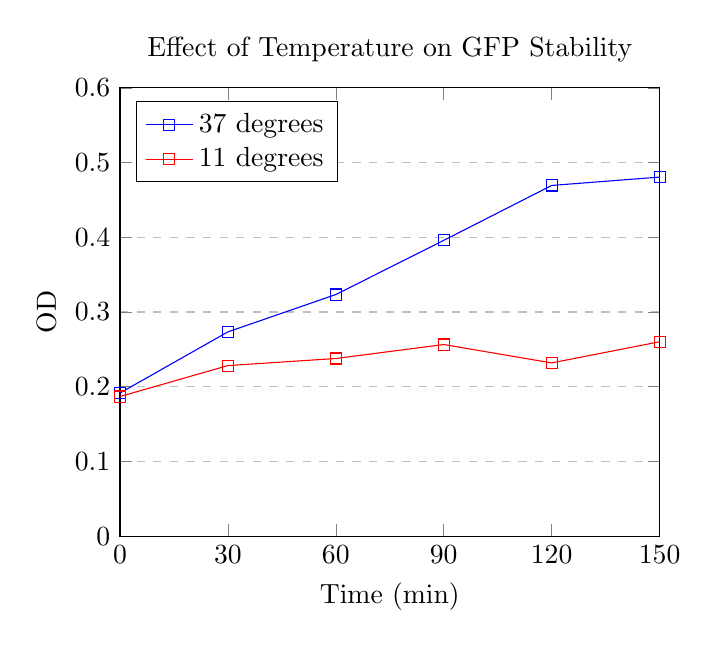
\begin{tikzpicture}
    \begin{axis}[
        title={Effect of Temperature on GFP Stability},
        xlabel={Time (min)},
        ylabel={OD},
        xmin=0, xmax=150,
        ymin=0, ymax=0.6,
        xtick={0,30,60,90,120,150},
        ytick={0,0.1,0.2,0.3,0.4,0.5,0.6},
        legend pos=north west,
        ymajorgrids=true,
        grid style=dashed,
    ]
    
    \addplot[
        color=blue,
        mark=square,
        ]
        coordinates {
        (0,0.1916)(30,0.2734)(60,0.3234)(90,0.3959)(120,0.4694)(150,0.4806)
        };
        \addlegendentry{37 degrees}
    
    \addplot[
        color=red,
        mark=square,
        ]
        coordinates {
        (0,0.1869)(30,0.2283)(60,0.2378)(90,0.2565)(120,0.2319)(150,0.2602)
        };
        \addlegendentry{11 degrees}
    
    \end{axis}
\end{tikzpicture}

\textbf{Fluorescence Intensity measurements:}

\begin{tabular}{|c|c|c|}
    \hline
    Time (min) & 37 degrees & 11 degrees \\
    \hline
    0 & 20609 & 1880 \\
    30 & 27129 & 25249 \\
    60 & 31557 & 26592 \\
    90 & 37818 & 28059 \\
    120 & 44292 & 28547 \\
    150 & 45128 & 30483 \\
    \hline
    
\end{tabular}

\textbf{Fluorescence Intensity plot:}

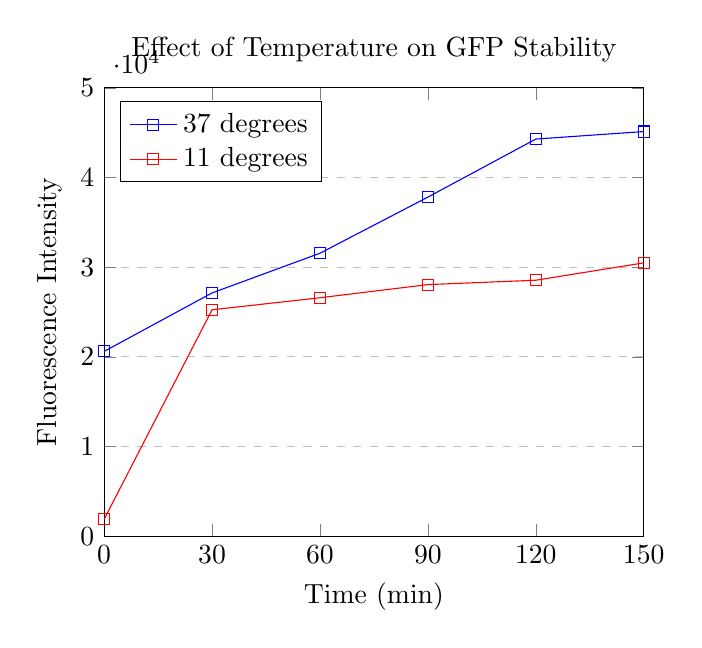
\begin{tikzpicture}
    \begin{axis}[
        title={Effect of Temperature on GFP Stability},
        xlabel={Time (min)},
        ylabel={Fluorescence Intensity},
        xmin=0, xmax=150,
        ymin=0, ymax=50000,
        xtick={0,30,60,90,120,150},
        ytick={0,10000,20000,30000,40000,50000},
        legend pos=north west,
        ymajorgrids=true,
        grid style=dashed,
    ]
    
    \addplot[
        color=blue,
        mark=square,
        ]
        coordinates {
        (0,20609)(30,27129)(60,31557)(90,37818)(120,44292)(150,45128)
        };
        \addlegendentry{37 degrees}
    
    \addplot[
        color=red,
        mark=square,
        ]
        coordinates {
        (0,1880)(30,25249)(60,26592)(90,28059)(120,28547)(150,30483)
        };
        \addlegendentry{11 degrees}
    
    \end{axis}
\end{tikzpicture}

\textbf{Fluorescence per cell intensity:}

\begin{tabular}{|c|c|c|}
    \hline
    Time (min) & 37 degrees & 11 degrees \\
    \hline
    0 & 107562.6 & 101016.6 \\
    30 & 99228.24 & 110595.7 \\
    60 & 97578.85 & 111825.1 \\
    90 & 95524.12 & 109391.8 \\
    120 & 94358.76 & 123100.5 \\
    150 & 93899.29 & 117152.2 \\
    \hline
    
\end{tabular}

\textbf{Fluorescence per cell intensity plot:}

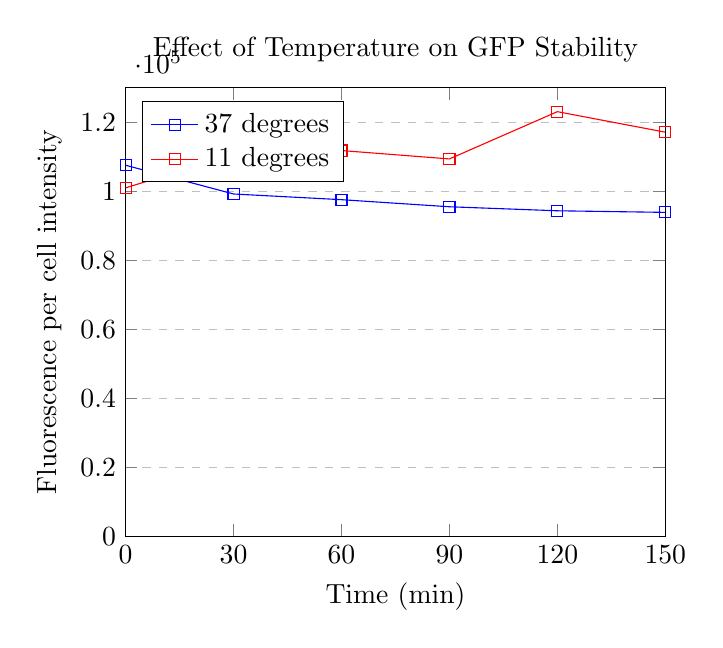
\begin{tikzpicture}
    \begin{axis}[
        title={Effect of Temperature on GFP Stability},
        xlabel={Time (min)},
        ylabel={Fluorescence per cell intensity},
        xmin=0, xmax=150,
        ymin=0, ymax=130000,
        xtick={0,30,60,90,120,150},
        ytick={0,20000,40000,60000,80000,100000,120000},
        legend pos=north west,
        ymajorgrids=true,
        grid style=dashed,
    ]
    
    \addplot[
        color=blue,
        mark=square,
        ]
        coordinates {
        (0,107562.6)(30,99228.24)(60,97578.85)(90,95524.12)(120,94358.76)(150,93899.29)
        };
        \addlegendentry{37 degrees}
    
    \addplot[
        color=red,
        mark=square,
        ]
        coordinates {
        (0,101016.6)(30,110595.7)(60,111825.1)(90,109391.8)(120,123100.5)(150,117152.2)
        };
        \addlegendentry{11 degrees}
    
    \end{axis}
\end{tikzpicture}

\textbf{Western Blotting:}
The results from Western Blotting confirmed the presence of GFP in the purified protein sample.
The membrane showed a single band at the expected molecular weight of GFP (27 kDa), indicating the successful purification of the protein.

\begin{figure}[H]
    \centering
    \includegraphics[width=0.4\textwidth]{Westernblot.jpg}
    \caption{Western blotting of purified GFP}
    \label{fig:Western_blot_image}
\end{figure}

\subsection*{Discussion}
From the results, we can conclude that the expression of our GFP at 11 degrees was successful. 
Doing this has increased our yeild as opposed to expressing at 37 degrees as has been confirmed by the \textit{effect of temperature studies}.
This is because the chaperones present in the BL21 Arctic Express$^{TM}$ cells which are cold-adapted-chaperones (cpn10, cpn60) help in the proper folding of the GFP protein at lower temperatures.
At higher temperatures, the GFP protein is more prone to denaturation and aggregation, leading to a decrease in fluorescence per cell intensity 
eventhough it has higher OD. This may be due to the fact that the GFP protein is not properly folded at higher temperatures and hence the fluorescence per cell intensity is lower.

The use of Ni-NTA affinity chromatography has been robust in purifying the GFP protein.
The presence of His-tag in the GFP protein has helped in the purification process.
The His-tag was lined to the protein via a TEV protease cleavage site which could also have been used to cleave the His-tag from the protein.
Non specific binding of proteins was removed by washing the column with wash buffer A and B, which is evident from the SDS-PAGE gel.

The Bradford assay has confirmed that the concentration of the purified GFP is 1.237 $\mu$g/ul.
This is a reasonable concentration for the GFP protein and can be used for further studies.

The SDS-PAGE and Western Blotting have confirmed the presence of GFP in the purified protein sample.
The SDS-PAGE gel showed a single band at the expected molecular weight of GFP (27 kDa), indicating successful purification of the protein.

The presence of another bands at a higher molecular weight in the SDS-PAGE gel can be due to aggregation or incomplete denaturation of the protein.

The Western Blotting has confirmed the presence of GFP in the purified protein sample.
The membrane showed a single band at the expected molecular weight of GFP (27 kDa), indicating the successful purification of the protein.


\subsection*{Conclusion}
The completion of this lab project involving the recombinant expression, purification, 
and primary characterization of the Green Fluorescent Protein (GFP) has provided valuable 
insights into the processes of protein production and analysis. Through recombinant expression, 
we successfully engineered cells to produce GFP, a widely used reporter protein with diverse 
applications in molecular and cellular biology. The purification process, utilizing affinity 
chromatography, allowed for the isolation of highly pure GFP protein from complex cellular lysates, 
demonstrating the efficacy of the purification protocol employed. Subsequent characterization of the 
purified GFP protein through SDS-PAGE and western blotting confirmed the successful expression and
purification of the protein.

The successful execution of this lab project not only deepened our understanding of recombinant protein expression and purification 
techniques but also equipped us with valuable skills applicable to a wide range of biochemical 
and biotechnological research endeavors. 

Overall, this lab project represents a significant step forward in our journey towards mastering fundamental 
techniques in biochemistry and molecular biology, paving the way for future exploration and innovation in the field.



\subsection*{Future Directions}
The success of this project lays the groundwork for further studies on GFP and other proteins.
The purified GFP can be used for various applications, including protein tagging, gene expression studies, and biological selections.
The effect of temperature on the stability of GFP can be further studied to understand the folding and stability of the protein.
The purified GFP can also be used to study its interaction with other proteins and ligands, providing insights into its biological functions.
The knowledge and skills gained from this project can be applied to the expression and purification of other proteins,
and can be used to further our understanding of protein structure and function.


\subsection*{Acknowledgements}
I would like to thank Prof. Mahipal Ganji for sparing his invaluable time and guiding me through this project.
I would also like to thank the lab instructor Dr. Varuna for her guidance and support throughout this project.
Her expertise and knowledge have been instrumental in the successful completion of this project.
A heartfelt thanks to our teaching assistant Vinod Sir for his constant care through every step of every protocol.

My sincere thanks to my lab mates for their support and encouragement throughout the project.
Their insights and suggestions have been invaluable in shaping the project and its outcomes.
Special thanks to Hemanya for the images, Vignesh for doing most of the experiments, Kalidas for the help with the time spent during incubations,
Adithya and Shloak for their help with graphs,tables and data analysis.

\subsection*{References}

\begin{enumerate}
    \item \url{https://www.news-medical.net/life-sciences/GFP-Applications.aspx}
    \item \url{https://www.explainthatstuff.com/luminescence.html}
    \item \url{https://goldbio.com/articles/article/how-does-iptg-induction-work}
    \item \url{https://qb3.berkeley.edu/education/lab-fundamentals-bootcamp/manual/proteins/protein-expression/}
    \item \url{https://bio.libretexts.org/Bookshelves/Biotechnology/Lab_Manual%3A_Introduction_to_Biotechnology/01%3A_Techniques/1.15%3A_SDS-PAGE}
    \item \url{https://www.ncbi.nlm.nih.gov/pmc/articles/PMC8969215/}
    \item \url{https://www.sinobiological.com/resource/protein-review/protein-purification-by-ac#:~:text=Ni-NTA%20Chromatography%20Purification%20Ni-NTA%20Agarose%20is%20an%20affinity,Cleared%20cell%20lysates%20are%20loaded%20onto%20the%20matrices.}
    \item \url{https://www.ncbi.nlm.nih.gov/pmc/articles/PMC3456489/}
    \item \url{https://microbeonline.com/western-blot-technique-principle-procedures-advantages-and-disadvantages/}
    \item \url{https://www.agilent.com/cs/library/usermanuals/Public/230191.pdf}
\end{enumerate}



\end{multicols}






\end{document}

